\documentclass[12pt, a4paper]{report}
% for guidance, see phd_work/mnras_guide.pdf
%\setlength\parindent{0pt}

\usepackage[english]{babel}
\usepackage[utf8x]{inputenc}
\usepackage[T1]{fontenc}

%\documentclass[useAMS,usenatbib]{mn2e}
\newcommand{\aap}{A\&A}
\newcommand{\araa}{ARAA}
\newcommand{\mnras}{MNRAS}
\newcommand{\apjl}{ApJL}
\newcommand{\apjs}{ApJS}
\newcommand{\apj}{ApJ}
\newcommand{\aj}{ApJ}
\newcommand{\nat}{Nature}
\newcommand{\pasa}{PASA}
\newcommand{\pasj}{PASJ}
\newcommand{\pasp}{PASP}
\newcommand{\aapr}{A\&AR}
\newcommand{\procspie}{Proc. SPIE}
\newcommand{\apss}{Ap\&SS}
%\newcommand{\rsquo}{`}

\usepackage{graphicx}
%\usepackage{braket}
\usepackage[english]{babel}
\usepackage{upgreek}
\usepackage{graphicx}
\usepackage{float}
\usepackage{natbib}
\usepackage{amsmath}
\usepackage{amssymb}
\usepackage{tabularx,ragged2e,booktabs,caption}
\usepackage{graphicx} % for images
\usepackage[font=small]{caption}
\usepackage{setspace}
\usepackage{epstopdf}
\usepackage{subcaption}

%%%%%%%%%%%	Page layout settings that follow JMU regulations     %%%%%%%%%%

\setlength{\hoffset}{0mm}
\setlength{\oddsidemargin}{0mm}
\setlength{\evensidemargin}{0mm}

\setlength{\voffset}{-10mm}
\setlength{\topmargin}{0mm}
\setlength{\headheight}{10mm}
\setlength{\headsep}{10mm}

\setlength{\textheight}{220mm}
\setlength{\textwidth}{155mm}

\setlength{\columnsep}{10mm}
\setlength{\marginparsep}{0mm}
\setlength{\marginparwidth}{0mm}
\setlength{\footskip}{20mm}

\setlength{\parindent}{0.3in} % Size of indent at the start of a new paragraph - originally 0.0in
\setlength{\parskip}{0.0in} % Spacing between paragraphs - originally 0.1in

\usepackage[hang,splitrule]{footmisc}

\addtolength{\footskip}{0.5cm}
\setlength{\footnotemargin}{0.3cm}
\setlength{\footnotesep}{0.4cm}

\makeatletter
\let\splitfootnoterule=\pagefootnoterule
\makeatother

%%%%%%%%%%%%%%%%%%%         Title Page            %%%%%%%%%%%%%%%%%%%%
\pagestyle{headings}

\begin{document}
\begin{titlepage}
\pagenumbering{arabic}

\vspace*{-0.4cm}

\begin{center}
\hrule
\vspace*{0.5cm}
{\Huge \sc Title \par}
\vspace*{0.5cm}
\hrule

\vspace*{5mm}
{\normalsize Report submitted for the application for transfer from M.Phil. to Ph.D.}

\vfill

{\bf Alexander Lisboa-Wright}

\end{center}

\vspace*{1.0cm}

\hrule
\vspace*{0.2cm}
\centering{Astrophysics Research Institute, Liverpool John Moores University}\\
\centering{September 2018}

\end{titlepage}

\begin{abstract}
The abstract of the paper.
\end{abstract}

\chapter{Introduction and background}
\section{Motivation}
The fundamental parameters of stars, such as their effective temperatures and metallicities, dictate their observed apparent properties, such as their luminosities and spectra. Hence, a full accounting of the effects of these parameters, and any physical stellar processes that impact on them, directly or indirectly, must be sought. ****Interior mixing is known to alter their 

\section{Thermohaline mixing}
The first months of the project were dedicated to the study of thermohaline mixing. The detailed study of this effect was begun by \cite{1972ApJ...172..165U} and \cite{1980A&A....91..175K}, to explain anomalous chemical abundances at the surface of mature (i.e., post-first-dredge-up (FDU)), ****low-mass ($\lesssim$ reld giant branch (RGB) stars. Specifically, the anomalies consist of an over-abundance of $^{12}$C, $^{16}$O and $^{14}$N, together with a paucity of $^{7}$Li and $^{1}$H, in the stellar spectra. Taken together, these particular changes in these particular species indicate an interaction between the RGB star's fusion shell and the surface, i.e. a mixing effect. Thermohaline mixing is proposed as a solution to this problem in the post-FDU phase in low-mass (< 1.5$M_{\odot}$) RGB stars****. The goal of this project is, ultimately, to implement a routine for calculating and propagating the effects of thermohaline mixing in BaSTI (\cite{2004ApJ...612..168P},\cite{2008ASPC..394..285P}), a 1D spherically-symmetric stellar interior model which produces both a detailed layered structural representation of a particular star at a series of ages in its lifetime and a summary of the most important fundamental properties, such as stellar mass, luminosity and radius, which are used to compare the models to observed properties of stars. The software can also use these models to produce isochrones at fixed metallicity \citep{2013A&A...558A..46P} with predicted magnitudes of stars of different masses in various filter systems.****

Mixing of material occurs due to local thermodynamic instabilities. For stars, this requires consideration of 4 thermodynamic quantities: pressure $P$, temperature $T$, density $\rho$ and molecular weight, $\mu$, as well as a coordinate system in which to operate. For simple stellar models, radial symmetry is assumed, allowing the system to be reduced to the radial coordinate $r$, measured from the stellar centre. If we assume a fully-ionized plasma containing $N$ atomic species, the local mean molecular weight can be calculated as:

\begin{equation}
\mu = \frac{1}{\sum_{i=1}^{i=N} (Z_{i}+1) \frac{X_{i}}{A_{i}}} \textnormal{,}
\label{mol_weight_def}
\end{equation}

where, for each species $i$, $Z_{i}$ is its proton number, $A_{i}$ its atomic mass number and $X_{i}$ its fraction by mass in the local region.

Let us consider a bubble of gaseous material in pressure-equilibrium with its surroundings and represent mixing as a significant change in the bubble's (radial) position on a significant time-scale, arising from small differences in the remaining 3 thermodynamic quantities between the bubble and its surroundings. For a non-rotating star, using a simple linear approach, together with the Archimedes principle, gives a set of 4 homogeneous differential equations for the (small) differences in $P$,$T$,$\mu$ and $r$ (Equations (3.1)-(3.4) in \cite{2017RSOS....470192S}). If $\Delta x_{i}$ are the differences in the 4 parameters, taking the ansatz form $\Delta x_{i} = B_{i} e^{nt}$ allows for a solution as a 3rd-order polynomial in $n$ (Equation (3.5) in \cite{2017RSOS....470192S}), if the determinant of the relevant matrix (dependent of the values of the $B_{i}$) is zero. The Routh-Hurwitz stability criterion can then be applied to this polynomial to give a general solution for $n$. For a physically-unstable solution, the exponent in the $\Delta x_{i}$ equation must be positive, i.e. $n$ must satisfy the condition $\operatorname{Re}(n) > 0$. Hence, the subsequent constraints on the polynomial coefficients form all the possible conditions for instability (at least one of which must be satisfied), and take the following form:

\begin{align}
\nabla _{\mu} &< 0 \label{mu_inv_ineq} \\
\nabla _{\textnormal{rad}} &> \nabla _{\textnormal{ad}} \label{schwarz_ineq} \\
\nabla _{\textnormal{rad}} &> \nabla _{\textnormal{ad}} + \left( \frac{\phi}{\delta} \right) \nabla _{\mu} \label{ledoux_ineq}
\end{align}

where $\nabla _{\mu} = d\ln\mu / d\ln P$, $\nabla _{\textnormal{rad}} = \left(\partial\ln T / \partial\ln P \right)_{\textnormal{rad}}$ and $\nabla _{\textnormal{ad}} = \left(\partial\ln T / \partial\ln P \right)_{\textnormal{ad}}$ are the temperature-pressure gradients for the local environment (dominated by radiation pressure) and the bubble (treated as an adiabatic ideal gas), respectively, $\phi = \left( \partial \ln\rho / \partial \ln\mu \right)_{P,T}$ and $\delta = -\left( \partial \ln\rho / \partial \ln T \right)_{P,\mu}$  \citep{1980A&A....91..175K}. For the case of this project****, $(\phi/\delta)$ is always positive, and has been assigned a value of 1.

%, but of different temperature and chemical composition,

For convection to occur in a given stellar region, only Equation (\ref{schwarz_ineq}), known as the Schwarzschild criterion for instability, needs to be true, as convection merely requires a non-zero $\Delta\mu$. Equation (\ref{ledoux_ineq}) is known as the Ledoux criterion. When there is a molecular weight inversion (thereby satisfying Equation (\ref{mu_inv_ineq})), instability arises invariably, but if only the Ledoux criterion is also true, the instability is thermohaline. If only the Schwarzschild criterion is true out of the three, the molecular weight gradient partially inhibits the effects of convective instability. The mixing process in this case is known as semiconvection \citep{2016ApJ...817...54M}.

%If both the other criteria are true, the Ledoux criterion is automatically satisfied, in the stellar case ($\nabla _{\textnormal{rad}},\nabla _{\textnormal{ad}} > 0$).

The basic structure of low-mass  RGB stars, starting from the physical centre of the star, can be summarised as follows:

\begin{enumerate}
\item Inert, electron-degenerate $^{4}$He-dominated core (98$\%$ by mass), generally extending out to a coordinate fractional mass of ~0.28$M_{\star}$.
\item Fusion shell, in which the fusion reactions which previously occurred in the main-sequence core occur now in the RGB phase. The main reactions are the pp-chain and CNO cycle.
\item Radiative zone, consisting of layers for which the none of the instability criteria are fulfilled, thus ensuring stability against convection. For a solar-mass RGB star, this extends out to ~0.29$M_{\odot}$, as calculated both in the model generated for this work by BaSTI  and by \cite{2006Sci...314.1580E}, who employed a fully-3D hydrodynamic approach.
\item Convective zone, where the Schwarzschild criterion is fulfilled, and mixing is modelled using the mixing-length theory (MLT)****ref, with the free parameter modelled such that, given solar input parameters, the model produces solar outputs. ****Given the extremely short characteristic timescales for convective mixing, this process can be assumed to be instantaneous in full-stellar modelling.
\item Atmosphere, where the radiation is emitted from the star - this layer consequently dominates the nature of the emission ($T_{\textnormal{eff}}$, emission lines, etc.)
\end{enumerate}

Thermohaline mixing, as noted above, requires a molecular weight inversion. Due to the $^{3}\textnormal{He}(^{3}\textnormal{He},2^{1}\textnormal{H})^{4}\textnormal{He}$.

Thermohaline mixing can be defined as a diffusive process \citep{1980A&A....91..175K}, so it can be constructed in models to obey the diffusion equation for the mass fraction of atomic species $i$, $X_{i}$, as follows****:

\begin{equation}
\frac{\partial X_{i}}{\partial t} = \frac{1}{\rho r^{2}}\frac{\partial}{\partial r} \left( \rho r^{2} D \frac{\partial X_{i}}{\partial r} \right)
\label{diffusion_eq}
\end{equation}

The strength of different diffusive effects in Equation (\ref{diffusion_eq}) is dictated by their respective diffusion coefficient $D$. In the case of thermohaline mixing, the coefficient is defined \cite{2010A&A...521A...9C} as:

\begin{equation}
D_{\textnormal{thl}} = C_{\textnormal{thl}} K \left( \frac{\phi}{\delta} \right) \frac{\nabla _{\mu}}{\nabla _{\textnormal{rad}} - \nabla _{\textnormal{ad}}}
\label{Dthl_def}
\end{equation}

where $C_{\textnormal{thl}}$ is a free parameter, which is set in this work to a value of $C_{\textnormal{thl}} = 1000$, a value which gives consistency between the results of modelling the diffusion equation and observations of field \citep{2007A&A...467L..15C} and globular cluster (\cite{2011ApJ...728...79A}, \cite{2012ApJ...749..128A}) stars and $K$ is the thermal diffusivity \citep{2017RSOS....470192S}, defined as:

\begin{equation}
K = \frac{4acT^{3}}{3\kappa\rho ^{2}c_{P}}
\label{diffusivity_def}
\end{equation}

where $a$ is the radiation constant, $c$ the speed of light, $\kappa$ the Rosseland mean opacity and $c_{P}$ the specific heat at constant pressure.
Given the requirement for a molecular-weight inversion, $D_{\textnormal{thl}}$ was set to zero if the local region 



%\begin{equation}
%
%\label{del_mu_def}
%\end{equation}


\section{Differential extinction}
Extinction of light between a source object, such as a star, and a remote observer is subject to various quantities, such as the density and metallicity of the interstellar medium along the emission travel path. Bolometric corrections represent mathematical estimates which account for the fact that, in a given filter, any part of the stellar spectrum outside the filter's wavelength range remains undetected by that filter. They are useful in all observations, in particular when observing objects visible only in a narrow spectral region.

After accounting for a general extinction effect on an object's emission, its apparent magnitude in a given filter $X$ (i.e. wavelength range, which we define as increasing from $\lambda _{1}$ to $\lambda _{2}$) is given by:

\begin{equation}
m_{X} = -2.5 \log_{10} \left(\frac{ \int_{\lambda_{1}}^{\lambda_{2}} f_{\lambda} \left( 10^{-0.4 A_{\lambda}} \right) S_{\lambda} d\lambda }{ \int_{\lambda_{1}}^{\lambda_{2}} f_{\lambda}^{0} S_{\lambda} d\lambda }\right) + m_{X}^{0}
\label{app_mag_def}
\end{equation}

where $f_{\lambda}$ represents the monochromatic flux at a given wavelength $\lambda$ at the observer distance, $A_{\lambda}$ is the extinction value as a function of wavelength, $S_{\lambda}$ is the response function and $f_{\lambda}^{0}$ and $m_{X}^{0}$ represent the monochromatic flux and apparent magnitude, respectively, of a known reference object in $X$. In this project,the star Vega was used as the reference.

Since our goal, ultimately, is to document potential effects of fundamental stellar properties upon observables, we need to connect the observational and idealised scenarios, for which we use bolometric corrections. For a filter $X$, the extinction parameter $A$ must be ****calibrated relative to a known value. For this reference, in this work we will input a value of the extinction in the well-studied Johnson-$V$ filter.
To derive the equation linking a bolometric correction with the extinction parameter, we start with the definition of a bolometric correction in $X$, $BC_{X}$:

\begin{equation}
BC_{X} \equiv M_{\textnormal{bol}} - M_{X}
\label{BC_def}
\end{equation}

where $M_{X}$ is the absolute magnitude of the object in $X$ and $M_{\textnormal{bol}}$ is its (predicted) absolute bolometric magnitude, defined relative to the Sun using:

\begin{equation}
M_{\textnormal{bol}} = M_{\textnormal{bol},\odot} - 2.5 \log_{10} \left( \frac{4\pi R^{2}F_{\textnormal{bol}}}{L_{\odot}} \right)
\label{mbol_sun}
\end{equation}

where  $F_{\textnormal{bol}}$ is the bolometric stellar flux at its surface, $R$ is the stellar radius, $M_{\textnormal{bol},\odot}$ is the solar absolute bolometric magnitude, ****which is assumed in this work to have a value of 4.75 and $L_{\odot}$ is the solar luminosity, for which a value of $3.844 \times 10^{33}$ erg s$^{-1}$ is used. Bolometric corrections can be expressed as a function of extinction using the universal definition of $M_{X}$ in terms of $m_{X}$ and the distance $d$ to the source:

\begin{equation}
M_{X} = m_{X} - 2.5 \log_{10}\left( \left( \frac{d}{10 \textnormal{pc}} \right)^{2} \right),
\label{abs_mag_def}
\end{equation}

together with the equation $f_{\lambda}d^{2}=F_{\lambda}R^{2}$, where $F_{\lambda}$ is the monochromatic flux at $\lambda$ at the stellar surface. This gives the final function for a bolometric correction:

\begin{align}
BC_{X} &= M_{\textnormal{bol},\odot} - m_{X}^{0} - 2.5 \log_{10} \left( \frac{4\pi R^{2}F_{\textnormal{bol}}}{L_{\odot}} \right) \\ &+ 2.5 \log_{10} \left( \frac{\int_{\lambda_{1}}^{\lambda_{2}} F_{\lambda} \left( 10^{-0.4 A_{\lambda}} \right) S_{\lambda} d\lambda}{\int_{\lambda_{1}}^{\lambda_{2}} f_{\lambda}^{0} S_{\lambda} d\lambda} \right)
\label{BC_extinc}
\end{align}

%With the effects of extinction included, the bolometric correction with a given extinction reference, $A_{r}$, is given by:

To extract the extinction parameter $A$****, we use the simple relation:

\begin{equation}
A_{X} = \left( \frac{A_{X}}{A_{V}} \right) A_{V}
\label{ratio_eq}
\end{equation}

together with the chosen value of $A_{V}$ (for this project the values were $A_{V} =$ 0, 1 - note that $BC_{X}(A_{V}=0)$  effectively assumes no extinction), before taking the difference between the two $BC_{X}(A_{V})$, giving the following equation:

\begin{align}
BC_{X}(0) - BC_{X}(A_{V}) &= \\ 2.5 \log_{10} \left( \frac{\int_{\lambda_{1}}^{\lambda_{2}} F_{\lambda}  S_{\lambda} d\lambda}{\int_{\lambda_{1}}^{\lambda_{2}} F_{\lambda}\left( 10^{-0.4 \left(A_{X,\lambda}/A_{V}\right)A_{V}} \right) S_{\lambda} d\lambda} \right)
\\ &= \left(A_{X}/A_{V}\right)A_{V}
\label{BCs_diff}
\end{align}

**** if $A_{X,\lambda}$ is assumed to constant within the wavelength range of each filter $X$, which is a valid assumption, even for the (wide-field) Hubble filters being studied in this work (Girardi****).

ATLAS9****

\chapter{Current state of the field}
\section{Thermohaline mixing}
Multiple**** studies have established the feasibility of thermohaline mixing in low-mass RGB stars from molecular mass gradient inversions as small as $(\Delta\mu / \mu) \sim$ 10$^{-4}$ (\cite{2006Sci...314.1580E}, \cite{2010ApJ...723..563D}). There were 2 slightly different approaches put forward for modelling thermohaline mixing:****
\begin{enumerate}

\item Linear theory \citep{1972ApJ...172..165U} - in a similar vein to the convection MLT, a simple linear model is assumed, one of the core assumptions being that the mixing occurs via radial movement of very thin regions (i.e. high aspect ratios). This allows the models of the mixing to remain one-dimensional and thus simplifies the calculation. The associated free parameter ($C_{thl}$) constrained by observation examples.
\item Blob theory \citep{1980A&A....91..175K} - the same as the linear theory, with the exception of the elimination of the assumption that the blob of chemically-different material is narrow. This allows for non-linear effects to be considered, including flow patterns which cause the moving blob to mix into its surroundings, reducing and eventually removing the blob as a distinct object.
\end{enumerate}

The difference between these two approaches, despite their identical underlying physical origin, was illustrated by \cite{2010ApJ...723..563D}, in which 

\section{Differential extinction}
Many papers ****(such as ?) have examined the effects of extinction from multiple perspectives, many by examining ratios of reddening (a.k.a. colour excess) values as functions of wavelength primarily. The seminal work in this field is \cite{1989ApJ...345..245C}, hereafter CCM, which avoided the complications of using reddening (which is not itself intrinsic and whose implications be impacted by the choice of filters) by fitting average ratios of the extinction parameter itself to observational data from stars taken in the IR, optical \citep{1988ESASP.281b.215C} and UV \citep{1988ApJ...328..734F} spectral regions, as an empirical function of wavelength $\lambda$. They produced a basic universal equation of the form:

\begin{equation}
A_{\lambda}/A_{V} = a(x) + b(x)/R_{V},
\label{CCM_general}
\end{equation}

where $x \equiv 1/\lambda$ and $R_{V} \equiv A(V)/E(B-V)$. The total wavelength range was divided into 4 subranges, each with a governing pair of empirically-determined equations (to determine $a(x)$ and $b(x)$, respectively). The CCM model underpins more recent studies of intrinsic effects on extinction (\cite{2018MNRAS.479L.102C}, \cite{2008PASP..120..583G}), and provides the basis for the synthetic  $A_{X}/A_{V}$ dataset in this project.

ATLAS9 model atmosphere predictions, calculated for a given value of stellar metallicity $Z$ and a grid of 476 combinations of $T_{\textnormal{eff}}$ and log($g$) values \citep{2004astro.ph..5087C} were used as synthetic stellar observation events****

\cite{2018MNRAS.479L.102C}, hereafter CV18b ****use a similar approach to this project for the 3 Gaia filters, extending the approach employed with other filter systems in \cite{2018MNRAS.475.5023C}, hereafter CV18a, i.e. deriving bolometric data from a library of synthetic stellar model atmospheres, then fitting the data to a model function to estimate the behaviour of the extinction as a function of stellar parameters. There are key differences between the two projects, however. Firstly, CV18a,b used MARCS model atmospheres instead of ATLAS9. More importantly, the metallicity and, particularly, $T_{\textnormal{eff}}$ ranges covered by CV18a,b were smaller than the ones covered in this project. This makes the results of this project more applicable for a wider range of $T_{\textnormal{eff}}$ values and therefore stellar population ages, particularly for the youngest such examples, such as open clusters, as shown by comparing Figures \ref{BaSTI_coverage_16M} and \ref{BaSTI_coverage_10G}, which represent scenarios for open and globular clusters, respectively.

\chapter{Methodology} \label{Methodology}
\section{Thermohaline mixing}

For modelling thermohaline mixing, the BaSTI (\cite{2004ApJ...612..168P}) 1D full-star, full-lifespan stellar evolution FORTRAN code was used and modified to calculate the impact, on both local radial layers and the overall star, of adding the effect of thermohaline mixing, on both short- and long-term time-scales. The software iterates through a series of variable time-steps between different model stellar objects, starting at a pre-determined phase of the stellar evolution sequence. The software reads in a file containing a pre-determined set of initial conditions, including initial stellar mass, helium mass-fraction $Y$ and metallicity, as well as global settings, such as the total number of time-steps for which to generate models and whether to include different mixing effects. The mass fractions of the atomic species for the initial model (age, $t = 0$) were pre-calculated and stored in a separate file.
The object at each point in simulated time compromises a series of spherical layers, each with a local value of various physical parameters and of the mass fraction of all species being considered, representing the detailed physical and chemical structure of the stellar interior at that time.

So far in this project, the thermohaline mixing-related quantities were calculated using a routine separate from the main BaSTI code, which was run in its entirety prior to employing the thermohaline routine. In this routine, all single differentials in a given layer $k$ were calculated linearly as follows:

\begin{equation}
\frac{dy}{dx} = \frac{y_{k+1} - y_{k-1}}{x_{k+1} - x_{k-1}} \textnormal{,}
\label{dy/dx_iter}
\end{equation}

a form known as the central difference method.
To determine the potential for thermohaline mixing at a given model age, the abundances for all species in each layer were combined into a molecular weight value using Equation (\ref{mol_weight_def}), then combined with the pressure of the same layer to produce the $k$th-layer value of $\nabla_{\mu}$ via Equation (\ref{dy/dx_iter}). $D_{thl}$ was then calculated using Equation (\ref{Dthl_def}), with a fixed value of $(\phi/\delta) = 1$ and the other parameters obtained directly from the BaSTI model output tables. Equation (\ref{diffusion_eq}) was then used, together with Equation (\ref{dy/dx_iter}) using the right-hand bracketed terms collectively as $y$, to give the time differential of the mass fraction.**** Since this is merely a first-order approximation test of the feasibility for thermohaline mixing, and since the central difference method throws up the possibility of a result of zero for a solitary positive-$D_{\textnormal{thl}}$ layer, the $k$th-layer value of $D_{\textnormal{thl}}$ was used for the diffusion equation. The $k$th-layer value of the mass-fraction as a function of time was then calculated using the following linear iterative equation:

\begin{equation}
X_{i,n,k} = X_{i,n-1,k} + \delta t \left( \frac{\partial X_{i}}{\partial t}\right)_{k},
\label{iter_timeind}
\end{equation}

where $n$ is the time iterator, $\delta t$ is the time-step, with a fixed value of 500yr.

\section{Differential extinction}
When calculating the bolometric corrections, the reference values taken by the parameters for Vega were:
\begin{enumerate}
\item $m_{X}^{0} = 0.03$ for the Gaia filters
\item $m_{X}^{0} = 0.00$ for the Hubble WFC3 filters
\end{enumerate}

together with $M_{\textnormal{bol},\odot} = 4.75$. It should be noted that, during the final subtraction to obtain values of $A_{X}/A_{V}$, the $m_{X}^{0}$ and $M_{\textnormal{bol},\odot}$ values at both $A_{V}$ calibration values are the same, so the final results are unaffected by any calibration errors. The non-zero calibration value of $A_{V} = 1$ was chosen, as this allows for significant changes in $A_{X}/A_{V}$ from Equation (\ref{BCs_diff}), while also being close enough to zero to avoid significant changes in $A_{X}/A_{V}$ due to the Forbes effect \citep{2008PASP..120..583G}. Although the ATLAS9 minimum$T_{\textnormal{eff}}$ value is 3500K, due to a low-$T_{\textnormal{eff}}$ artefact present in the data for several filters in both the WFC3 and Gaia systems, this project only analysed data for $T_{\textnormal{eff}} \geq 4500$K. The total range of parameter values used in this project can be found in Table \ref{param_range_table}.

\begin{table}
\begin{tabular}{cccc}
\hline
Parameter & Minimum & Maximum & Number of values\\
\hline
$T_{\textnormal{eff}}$/K & 4500 & 50000 & 76 \\
log($g$/cm s$^{-1}$) & 0.0 & 5.0 & 11 \\
log($Z/Z_{\odot}$) & -2.0 & 0.5 & 4 \\
\hline

\end{tabular}
\caption{Stellar parameters used for calculating function in this project. Note: not all $T_{\textnormal{eff}}$ values have data for all log($g$) values - see \cite{2004astro.ph..5087C} for details}
\label{param_range_table}
\end{table}

This first fitting step was carried out assuming a function of $T_{\textnormal{eff}}$ only, with no anchor points, for  extinction data at a fixed value of stellar surface gravity (log($g$/cm s$^{-1}$) = 5.0) and metallicity ($Z = Z_{\odot}$). Coincidentally, this also avoid any impact of the aforementioned Forbes effect due to low-$T_{\textnormal{eff}}$ values (less than 4000K, becoming especially prominent at 2500K, according to \cite{2008PASP..120..583G}). The errors on the resulting values for the coefficients of $A_{1}$ were computed as a covariance matrix. The $\sigma$ values for the coefficients displayed in Table \ref{R1_coeffs_table} were extracted from the variances, which together form the leading diagonal of the covariance matrix. The results of this stage are stored in the function $A_{1} = A_{X}/A_{V}(T_{\textnormal{eff}})$. This function took on one of two function forms, each containing 3 free parameters (denoted by $a$,$b$ and $c$), depending on the relative performance of both functions in each filter. The first case, referred to in Table \ref{R1_coeffs_table} by the abbreviation `pow', models a fit of the following power-law form:

\begin{equation}
A_{1,\textnormal{pow}} (T_{\textnormal{eff}}) = a (T_{\textnormal{eff}})^{b} + c
\label{Teff_pow}
\end{equation}

while the second case (denoted by `exp') models an exponential:

\begin{equation}
A_{1,\textnormal{exp}} (T_{\textnormal{eff}}) = a \exp{(b T_{\textnormal{eff}})} + c
\label{Teff_exp}
\end{equation}

The second fitting, whose results are stored as $A_{2}(T_{\textnormal{eff}},\log{g})$ was treated as a correction to the results of the $A_{1}$ fitting. Not all filters required a second fitting, as seen in Table \ref{R2_yn_table}. Since the main variations generally arise from changes in $T_{\textnormal{eff}}$, the final output of results is a plot of $A_{X}/A_{V}$ against $T_{\textnormal{eff}}$. Given that the $A_{1}$ results remain consistent with the data at high $T_{\textnormal{eff}}$ values across all filters due to the data tending towards a constant value of $A_{X}/A_{V}$, an upper $T_{\textnormal{eff}}$-limit of 8000K was set for $A_{2}$ as an anchor point. The data for the fitting was obtained by taking the data used to fit $A_{1}$ ($Z = Z_{\odot}$, log($g$)=5.0) and subtracting from it the data at all other log($g$) values. The $A_{2}$ results****

Given the issues encoutered with modelling the $A_{2}$ functions, this project utilised the latest version of the BaSTI database \citep{2018ApJ...856..125H} to ascertain the range of log($g$) values covered by the selected $T_{\textnormal{eff}}$ range.

\chapter{Results so far}
\section{Thermohaline mixing}
Using the methodology described in Section \ref{Methodology} and the BaSTI model described in Table \ref{basti_params}, the thermohaline routine was applied to the output physical and chemical data at a model age of $\log_{10}(t/\textnormal{yr}) = 10.10616695$ in simulated time, for which $\log_{10}(L/L_{\odot}) = 2.1231$, at which point this star is in the RGB phase and has settled into equilibrium following the FDU. The species selected to trace the location and evolution of any thermohaline mixing event was $^{14}$N. This selection was made on the basis of known changes in $^{14}$N abundance as a function of temperature, and hence radius, within the fusion shell.

The radial gradients of all chemical species, the mean molecular weight, $\nabla_{\mu}$,  $D_{thl}$ and the time-evolution data for $X_{^{14}\textnormal{N}}$ were calculated for each layer. Focussing on the region of the hydrogen-burning shell, the $^{3}$He gradient is plotted against stellar radius in Figure \ref{dHe3/dr_colour}, with the line colour corresponding to the local value of $D_{thl}$, as shown in the colour bar. For a known fusion region, the positive value of $dX/dr$ for a given species indicates the burning of that species in one or more fusion mechanisms. The conclusion that can be drawn from Figure \ref{dHe3/dr_colour} is that the conditions required for thermohaline mixing (indicated by non-zero $D_{\textnormal{thl}}$) exist in the outer part of the $^{3}$He fusion region.

For the same radial region, the mass fraction for $^{14}$N is shown in Figure \ref{dXN14/dt_colour}, with each line representing the mass-fraction profile at a different time, with specific times listed in the legend. The behaviour of the mass fraction in the left-hand side of the figure ($R \lesssim 0.055R_{\odot}$) matches the behaviour shown in ****FigureX of ****paperY. The explanation for this two-step series is the domination of the CNO cycle in burning hydrogen in RGB fusion shells over the pp-chain, which dominates in MS core hydrogen burning. 

The CNO cycle in low-mass stars consists of two separate cyclic branches, which create**** $^{4}$He from $^{1}$H via two different series of proton captures and $\beta ^{+}$ decays involving isotopes of C, N and O as catalysts. Focussing specifically on $^{14}$N, which is a stable isotope, the difference in its interactions between the cycles is its parent nuclei. In the CN cycle-branch, it is produced via the $^{13}$C($^{1}$H,$\gamma$)$^{14}$N reaction. In the NO cycle-branch, it is produced via the $^{17}$O($^{1}$H,$^{4}$He)$^{14}$N. For each branch of the CNO cycle to be completed, it requires a temperature sufficiently high to support all its constituent fusion reaction steps. When this condition is no longer fulfilled, the production and destruction of the C, N and O isotopes is no longer in equilibrium. As temperature decreases moving radially outwards, the first branch to reach this stage is the NO cycle, followed by the CN cycle. Once this stage is reached, reaction rates dictate how elemental abundances change. The NO cycle, which produces $^{14}N$ overall, stops, such that $^{14}N$ abundance drops at lower temperatures. At temperatures too low to sustain the CN cycle, the $^{12}$C stops being fused**** and hence the production of nitrogen is halted.

This is an important observation as it establishes the location of $^{3}$He burning as being in the outer part of the H-burning shell, which agrees with the predictions of other models and is closest to the radiation zone, where thermohaline mixing is hypothesised to take effect. Figure \ref{dXN14/dt_colour} shows that, in a timespan of ~$5 \times 10^{4}$yr, of the order of the intervals between the ages of individual BaSTI models (~10$^{4}$yr around the model considered in the plots), the projected effect of thermohaline mixing on the local mass fraction of $^{14}$N is highly significant.


\begin{table}
\begin{tabular}{cc}
\hline
Input (initial) parameter & Value \\
\hline
Start time, ($t=0$) & pre-MS \\
Mass & 1$M_{\odot}$ \\
$Y$ & 0.248 \\
$Z$ & 0.0172 ($=Z_{\odot}$) \\
Diffusion & Enabled \\
\hline
\end{tabular}
\caption{BaSTI initial setup}
\label{basti_params}
\end{table}

\begin{figure}
\begin{center}
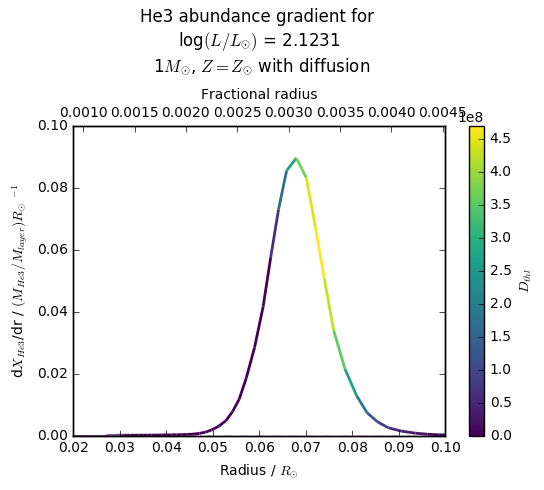
\includegraphics[scale=0.6]{../mu_test_data/mu_test_graphs/eq_logL=2p1231_He3_radius_gradient_Dthl_color.png}
\caption{$^{3}$He abundance gradient for model with $Z = Z_{\odot}$, $M = 1M_{\odot}$ and diffusion effects included, at a point $\log(L/L_{\odot}) = 2.1231$}
\label{dHe3/dr_colour}
\end{center}
\end{figure}

\begin{figure}
\begin{center}
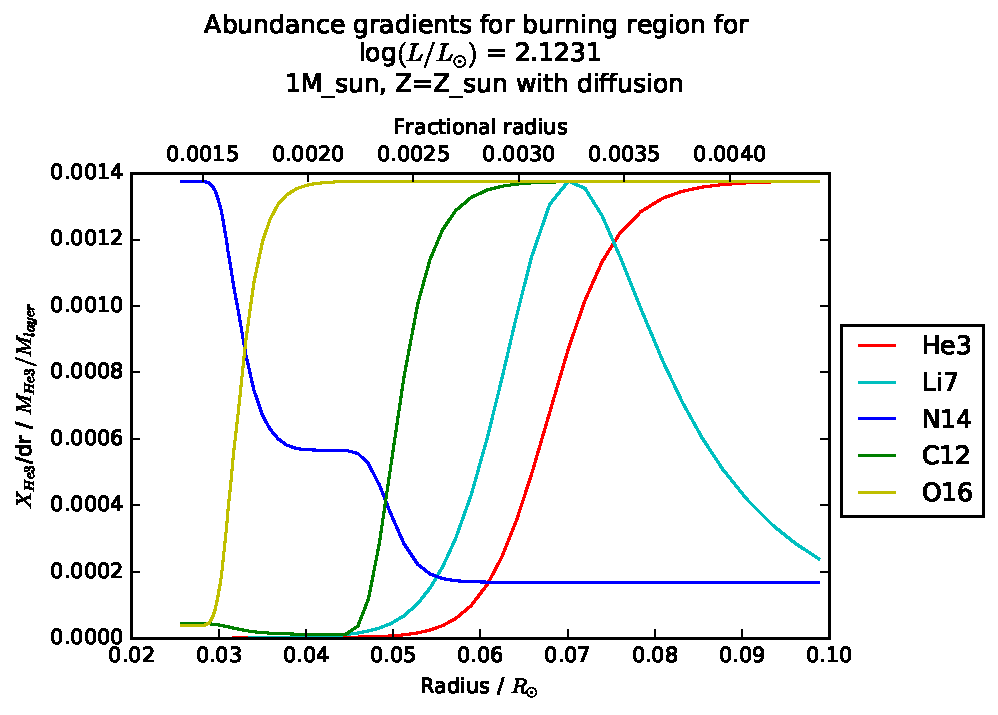
\includegraphics[scale=0.5]{../mu_test_data/mu_test_graphs/burning_logL=2p1231_5species.pdf}
\caption{Mass fractions, with values normalised to those for $^{3}$He, for 5 species for model with $Z = Z_{\odot}$, $M = 1M_{\odot}$ and diffusion effects included, at a point $\log(L/L_{\odot}) = 2.1231$}
\label{5specs_norm}
\end{center}
\end{figure}

\begin{figure}
\begin{center}
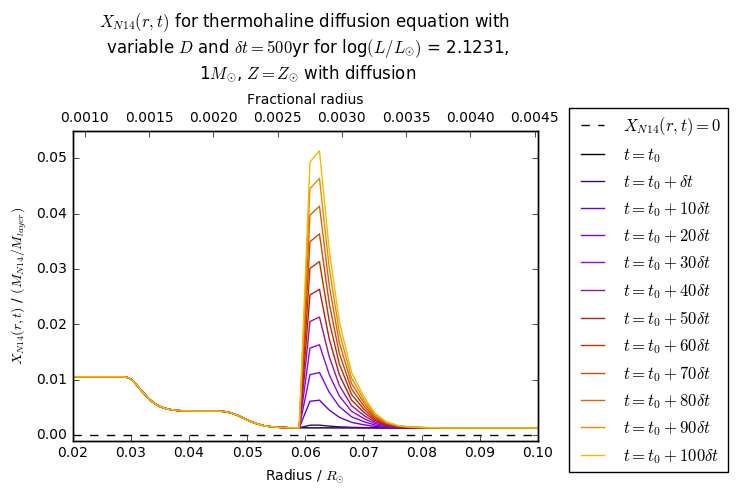
\includegraphics[scale=0.4]{../mu_test_data/mu_test_graphs/eq_logL=2p1231_time_diff_eq_Dvar_10dt_dmu_k_lim.png}
\caption{$^{14}$N abundance time derivative for model with $Z = Z_{\odot}$, $M = 1M_{\odot}$ and diffusion effects included, at a point $\log(L/L_{\odot}) = 2.1231$}
\label{dXN14/dt_colour}
\end{center}
\end{figure}

\section{Differential extinction}


Table \ref{R1_coeffs_table} shows the best results obtained for $A_{1,\textnormal{exp}} (T_{\textnormal{eff}})$ for all filters. All coefficient values are presented with a precision of 4 significant figures. 

\begin{table*}
\begin{tabular}{cccccc}
\hline
%\multirow{2}{*}{System} & \multirow{2}{*}{Filter} & \multirow{2}{*}{$A_{1}$ function} & \multicolumn{3}{c}{$A_{1}$ coefficients} \\ \cline{4-6}
%\textbf{Filter} \\
System & Filter & $A_{1}$ function & & $A_{1}$ coefficients & \\
 & & & $a$ & $b$ & $c$ \\
\hline
% -2.32428259e+02  -1.07634845e-03   2.93338391e+00
% -1.28482746e+02  -1.03094181e-03   2.61038997e+00
% -9.72567775e-01  -3.51770388e-04   2.06004238e+00
% -5.33470924e+05  -1.66350652e+00   2.05158490e+00
% -1.51556105e+04  -1.58229494e+00   1.64765130e+00
% -0.59910717 -0.08070638  1.73786479
% -9.99999999e+04  -1.78304457e+00   1.35186267e+00
% -1.20707226e+05  -1.70657822e+00   1.22045256e+00
% -4.59655266e+05  -1.88059297e+00   1.07985380e+00
% -3.13655088e+05  -1.82928924e+00   9.64793923e-01
% -5.47562323e+05  -2.02950259e+00   8.78683006e-01
% -6.32767059e+03  -1.57627077e+00   6.56703339e-01
% -3.72711692e+03  -1.43145264e+00   6.15752594e-01
% -3.38142759e+04  -1.39444200e+00   1.03998507e+00
% -457.55192948   -0.89995256    1.24675509
% -4.38278161e+03  -1.36062232e+00   6.77129794e-01
& f218w & exp & -232.4$\pm$48.1 & -(1.076$\pm$0.043)$\times 10^{-3}$ & 2.933$\pm$0.007 \\
& f225w & exp & -128.5$\pm$13.8 & -(1.031$\pm$0.022)$\times 10^{-3}$ & 2.610$\pm$0.003 \\
& f275w & exp & 0.9726$\pm$0.0581 & -(3.518$\pm$0.109)$\times 10^{-4}$ & 2.060$\pm$0.001 \\
& f300x & pow & -(5.335$\pm$0.936)$\times 10^{5}$ & -1.664$\pm$0.021 & 2.052$\pm$0.001 \\
& f336w & pow & -(1.516$\pm$0.723)$\times 10^{4}$ & -1.582$\pm$0.056 & 1.648$\pm$0.001 \\
& f390w & pow & -0.5991$\pm$0.1494 & -0.08071$\pm$0.09090 & 1.738$\pm$0.309 \\
WFC3 & f438w & pow & -(1.000$\pm$0.463)$\times 10^{5}$ & -1.783$\pm$0.054 & 1.352$\pm$0.001 \\
& f475w & pow & -(1.207$\pm$0.379)$\times 10^{5}$ & -1.707$\pm$0.037 & 1.220$\pm$0.001 \\
& f555w & pow & -(4.560$\pm$1.490)$\times 10^{5}$ & -1.881$\pm$0.038 & 1.080$\pm$0.001 \\
& f606w & pow & -(3.137$\pm$0.911)$\times 10^{5}$ & -1.829$\pm$0.034 & 0.9648$\pm$0.0003 \\
& f625w & pow & -(5.476$\pm$3.709)$\times 10^{5}$ & -2.030$\pm$0.079 & 0.8787$\pm$0.0002 \\
& f775w & pow & -(6.328$\pm$4.571)$\times 10^{3}$ & -1.576$\pm$0.085 & 0.6567$\pm$0.0001 \\
& f814w & pow & -(3.727$\pm$1.381)$\times 10^{3}$ & -1.431$\pm$0.044 & 0.6158$\pm$0.0002 \\ \hline
& G & pow & -(3.381$\pm$0.733)$\times 10^{4}$ & -1.394$\pm$0.026 & 1.040$\pm$0.001 \\
Gaia & G\textsubscript{bp} & pow & -457.6$\pm$64.9 & -0.9000$\pm$0.0172 & 1.247$\pm$0.002 \\
& G\textsubscript{rp} & pow & -(4.383$\pm$0.871)$\times 10^{3}$ & -1.361$\pm$0.023 & 0.6771$\pm$0.0002 \\ \hline

\end{tabular}
\caption{tgfdidgdi****}
\label{R1_coeffs_table}
\end{table*}

\begin{table*}
\begin{tabular}{ccc}
\hline
System & Filter & $A_{2}$ required? \\
\hline
& f218w & Y \\
& f225w & Y \\
& f275w & Y \\
& f300x & Y \\
& f336w & N \\
& f390w & N \\
WFC3 & f438w & N \\
& f475w & N \\
& f555w & N \\
& f606w & N \\
& f625w & N \\
& f775w & N \\
& f814w & N \\
\hline
& G & N \\
Gaia & G\textsubscript{bp} & N \\
& G\textsubscript{rp} & N \\ \hline

\end{tabular}
\caption{tgfdidgdi****}
\label{R2_yn_table}
\end{table*}

As shown in Figure****, for some filters, there are significant changes in the extinction ratio values at fixed $T_{\textnormal{eff}}$ ($|\delta A| > 0.02$), due to changes in log($g$), $Z$ or both. 

\begin{figure*}
\begin{center}
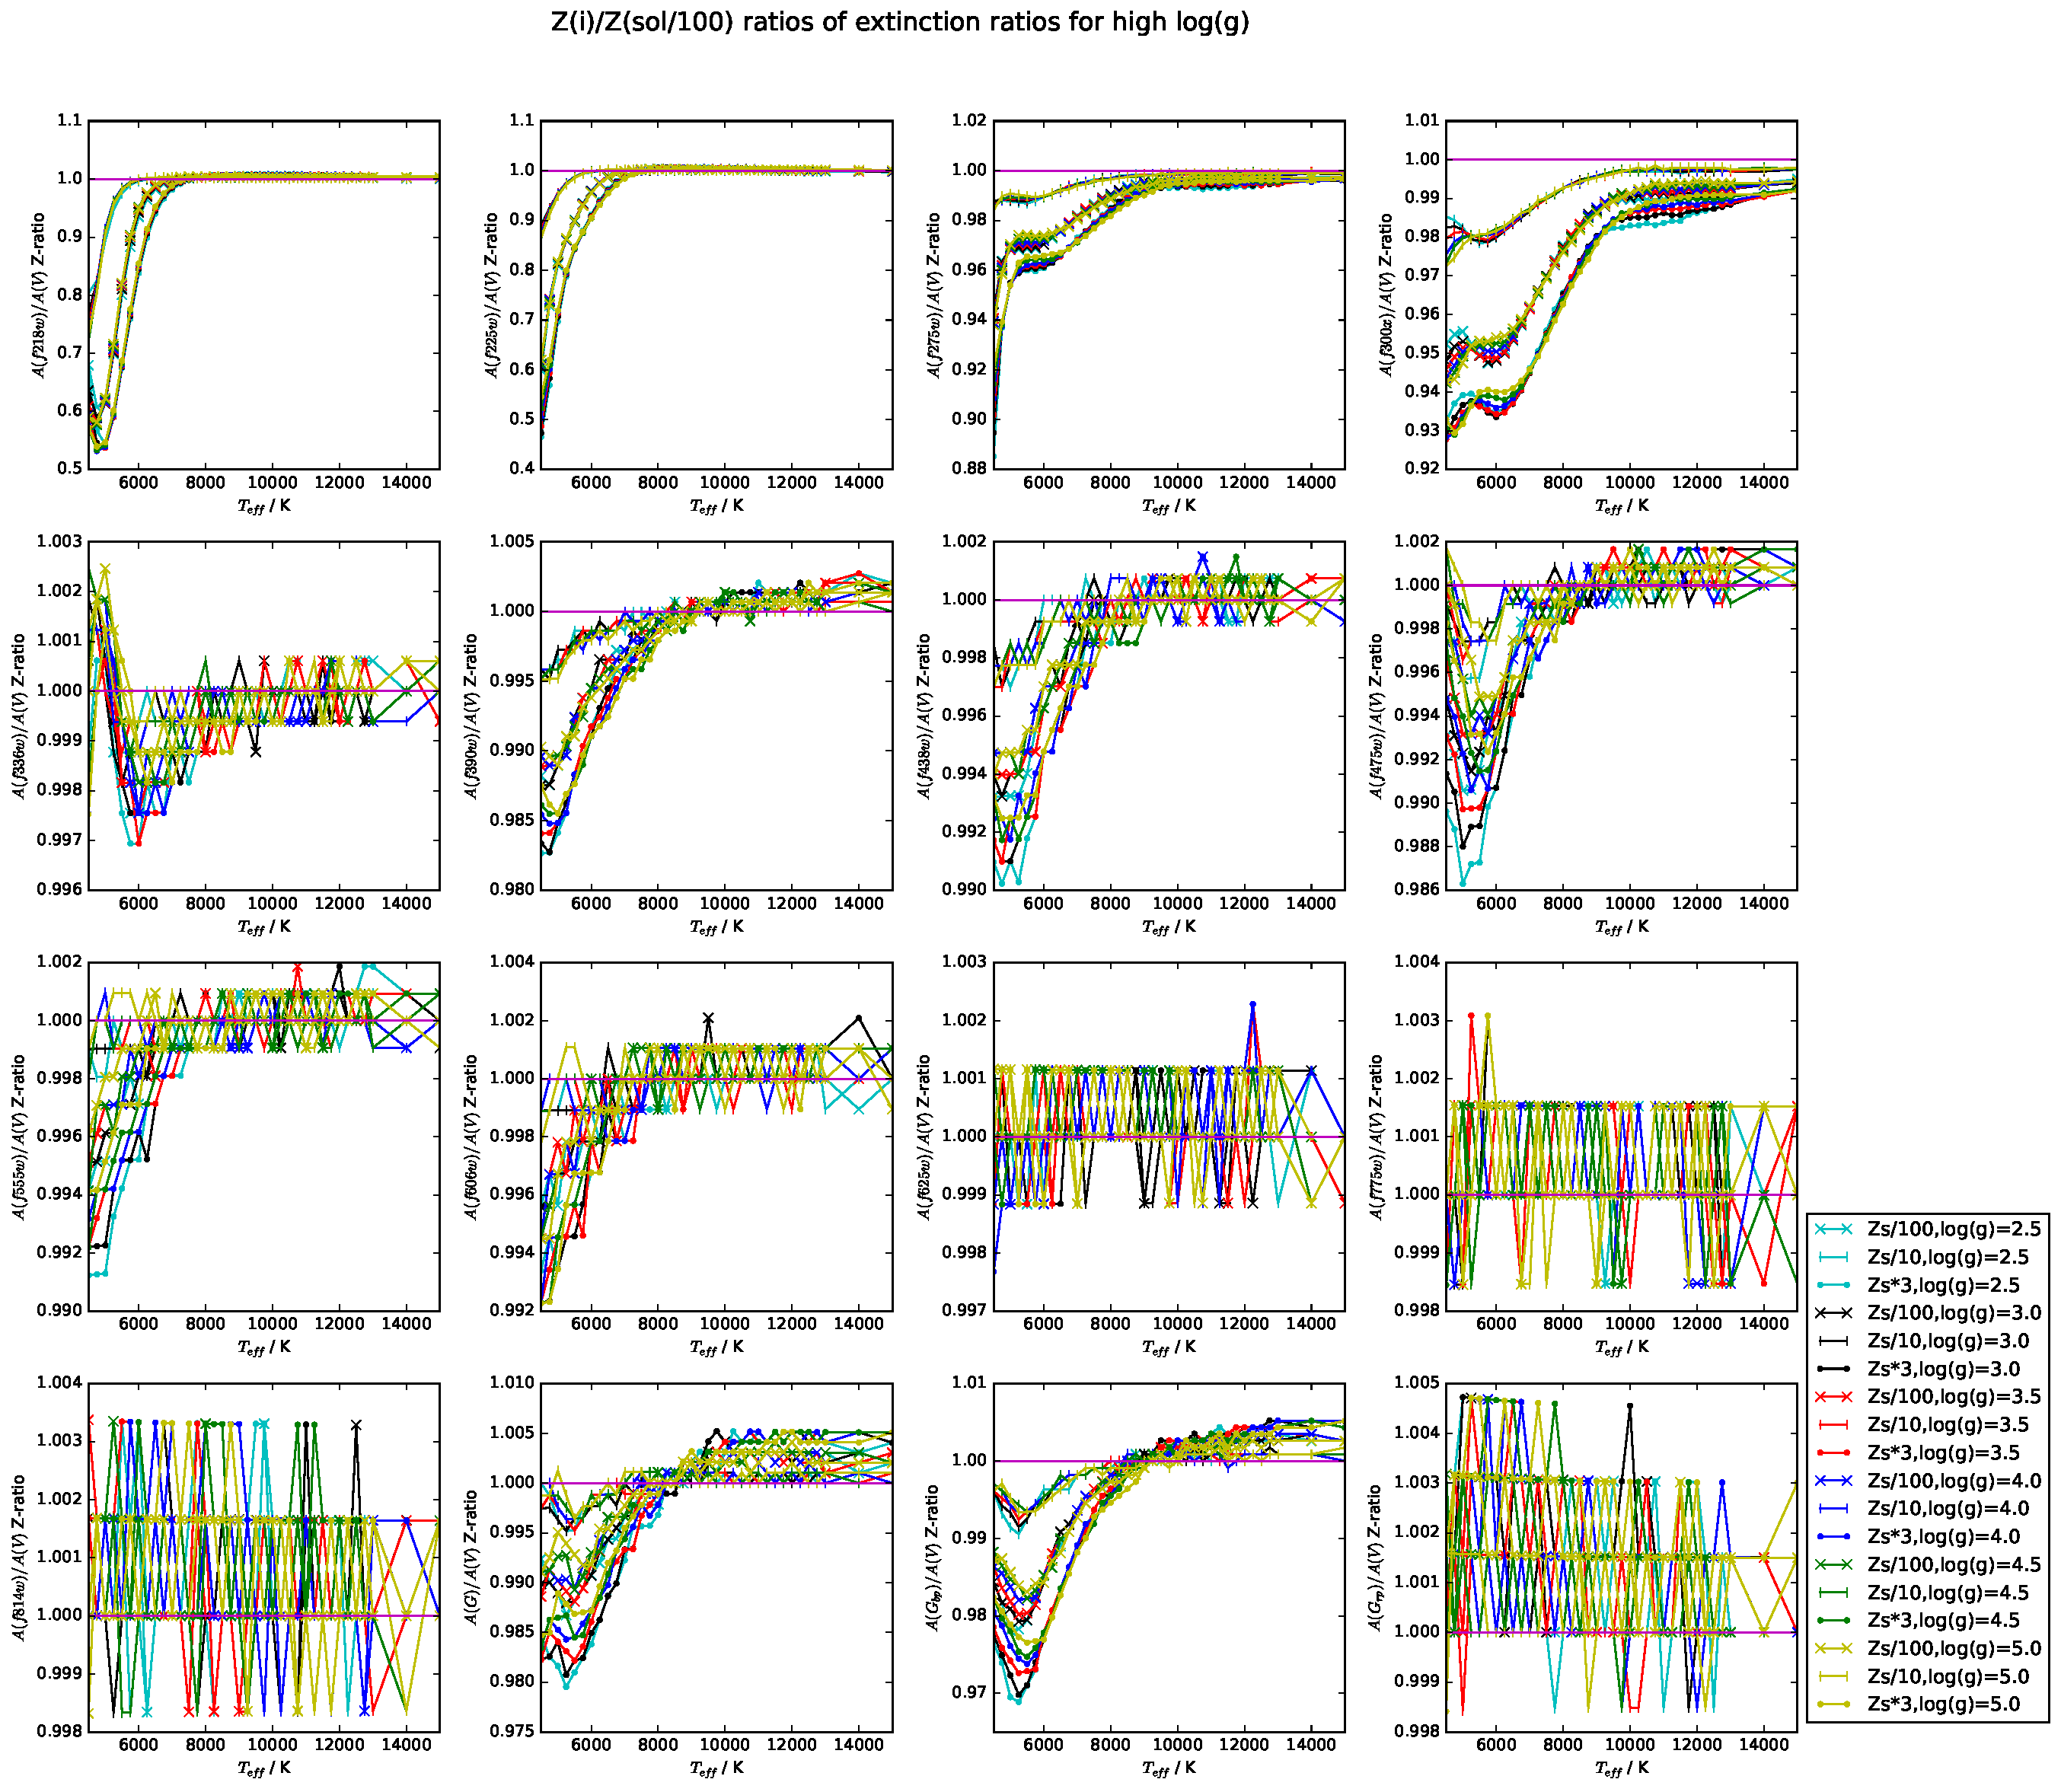
\includegraphics[scale=0.3]{../Aall_ratio_Zs_div_Z2_effect_high_logg_zoom_15000.pdf}
\caption{****psrsoft image output for a simulated pulsar data file}
\label{all_Z_Z2_ratio}
\end{center}
\end{figure*}

\begin{figure*}
\begin{center}
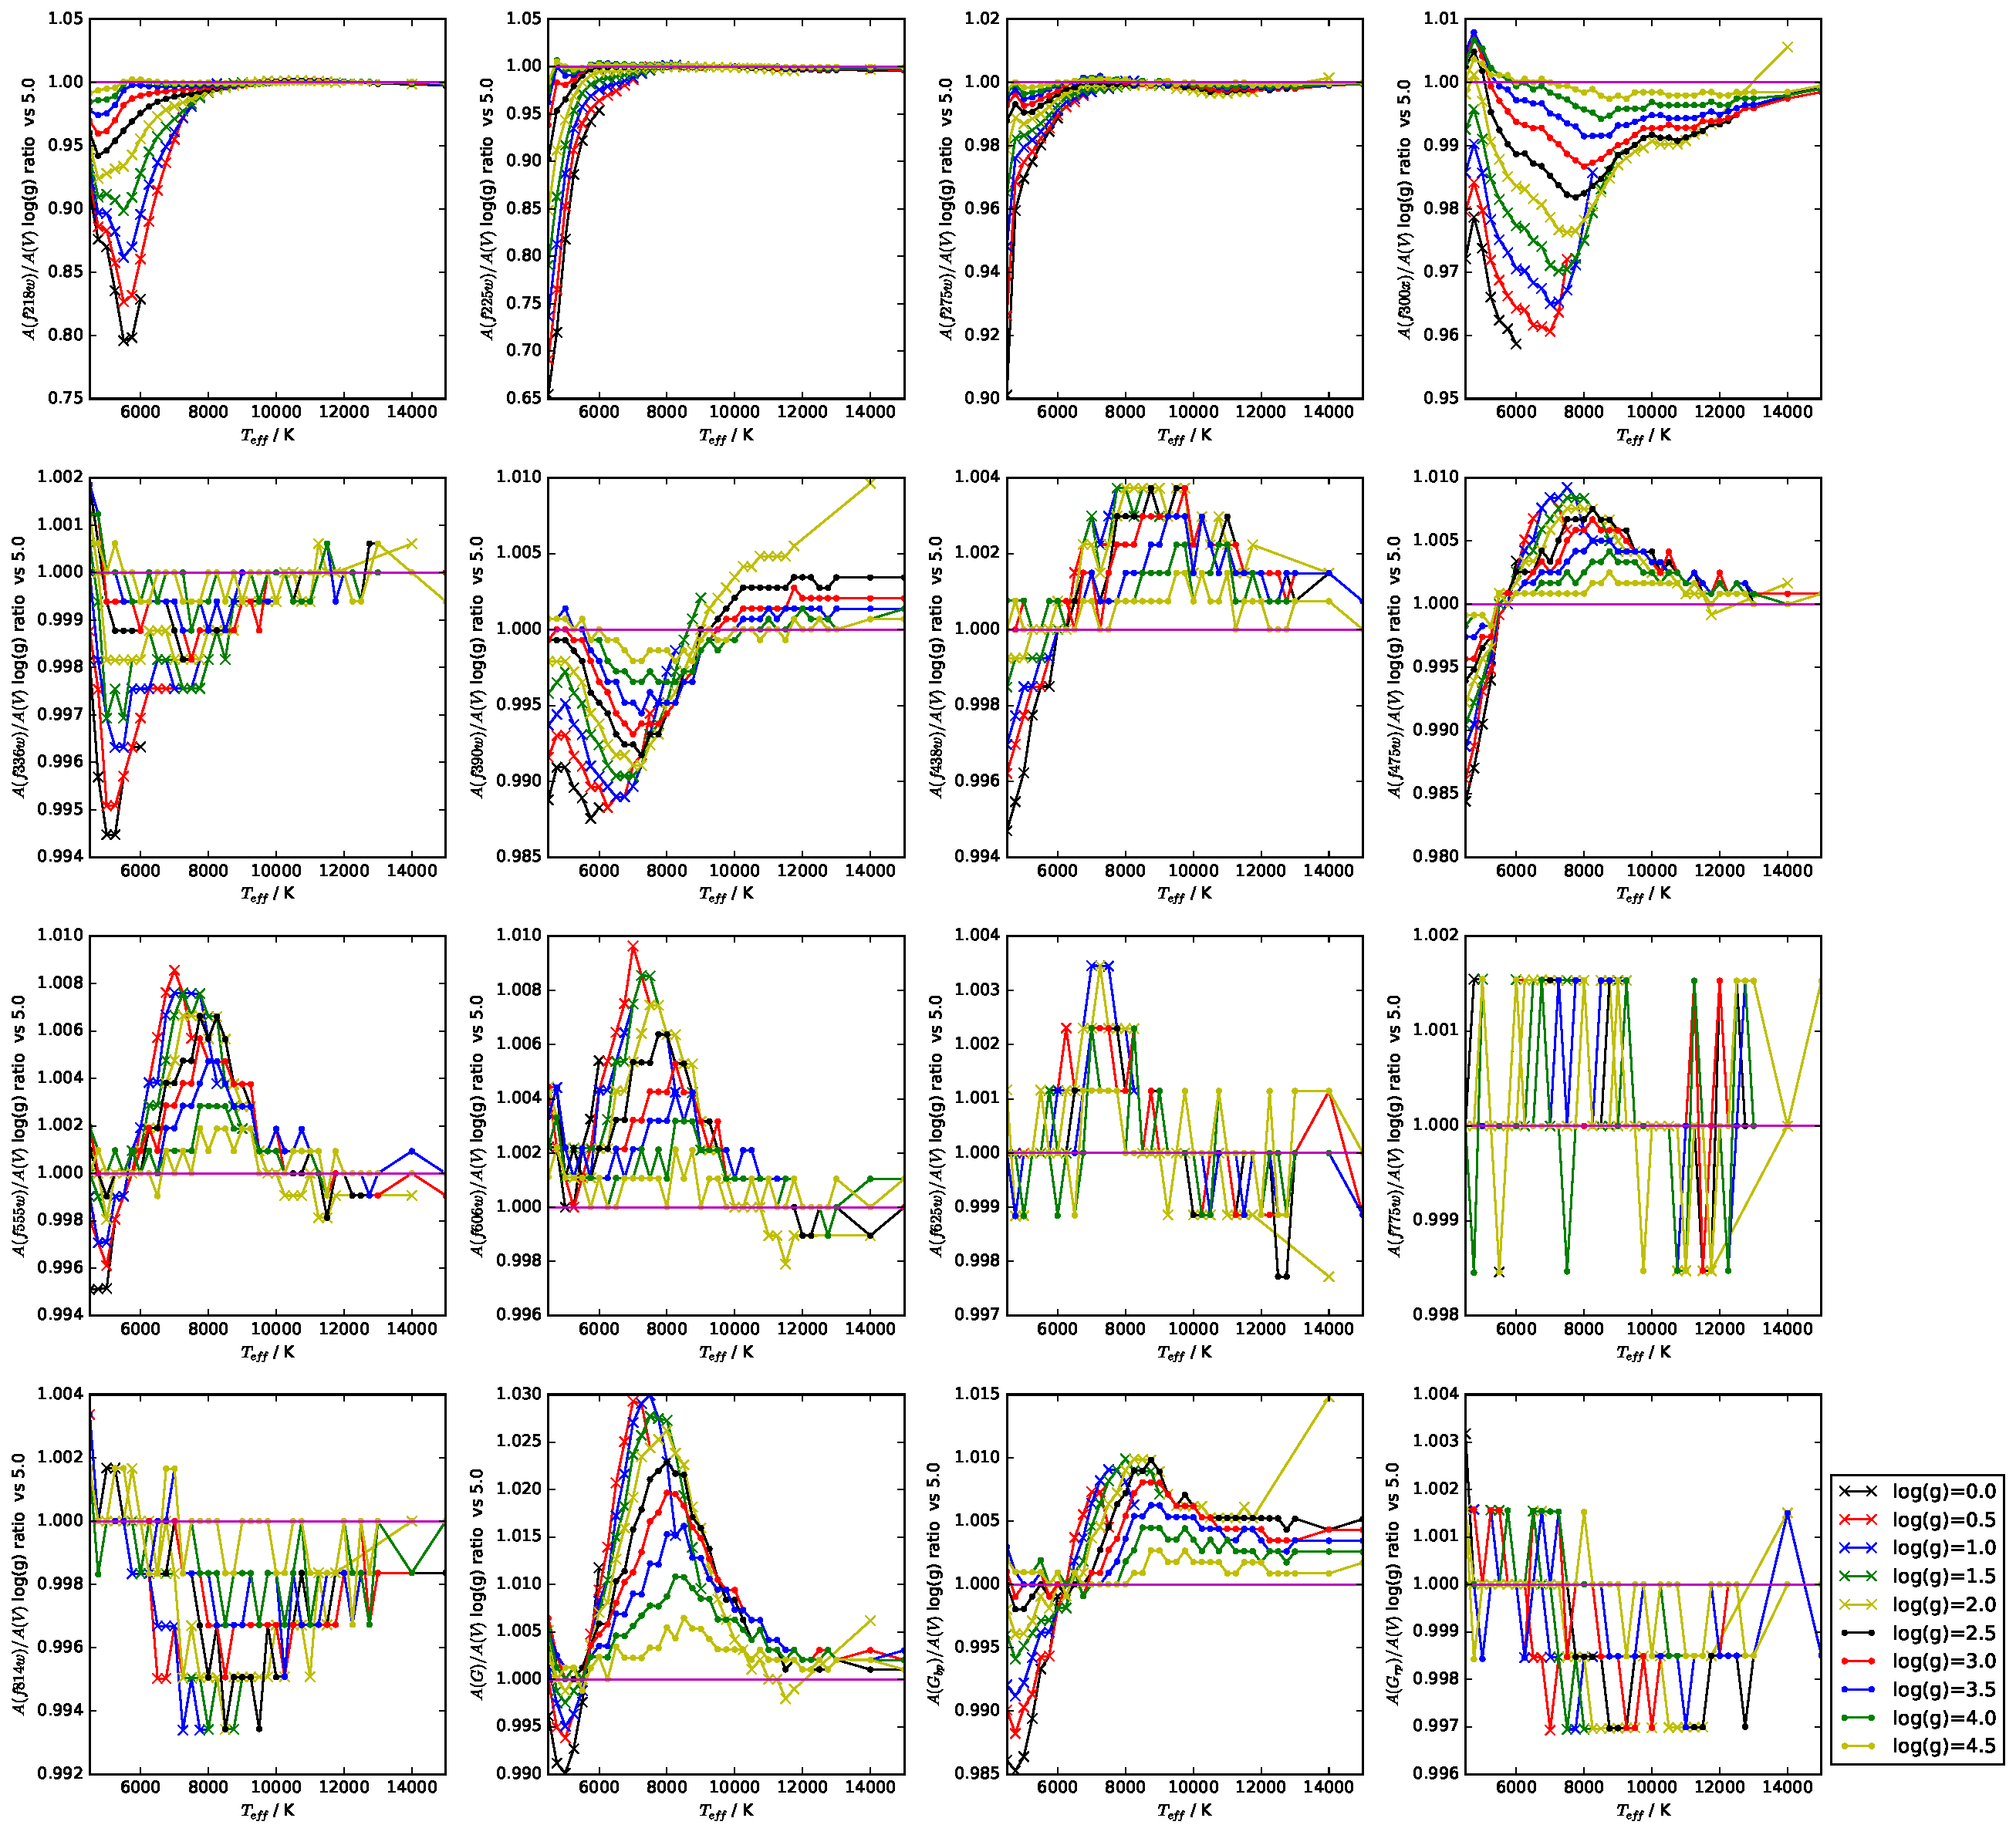
\includegraphics[scale=0.3]{../Aall_ratio_all_logg_div_5p0_effect.pdf}
\caption{Ratios of $A_{X}/A{V}$ values for different log($g$) values compared with log($g$)=5.0 data at solar metallicity}
\label{all_logg_logg5_ratio}
\end{center}
\end{figure*}

\begin{figure}
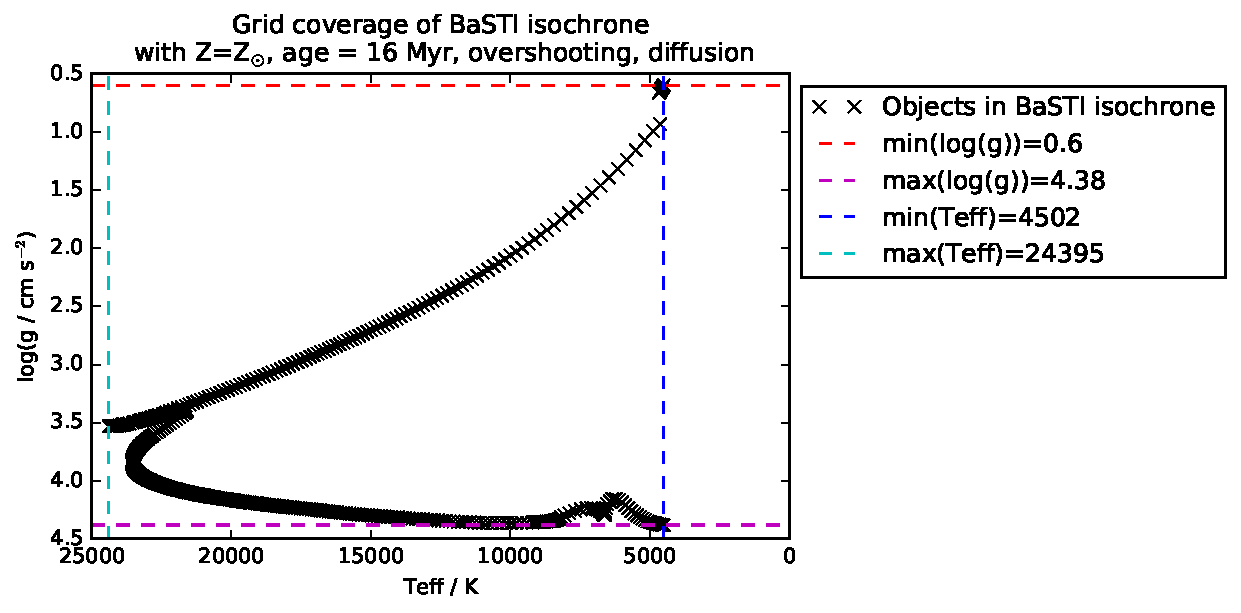
\includegraphics[scale=0.4]{../wfc3_16_23Myr_10Gyr_complex_solar/wfc3_ATLAS9_grid_BaSTI_coverage_c16_complex_Zsol_4500.pdf}
\caption{$T_{\textnormal{eff}}$-log($g$) grid coverage by a 16 Myr, $Z_{\odot}$ BaSTI isochrone ****including mass-loss, core overshooting and diffusion effects}
\label{BaSTI_coverage_16M}
\end{figure}

\begin{figure}
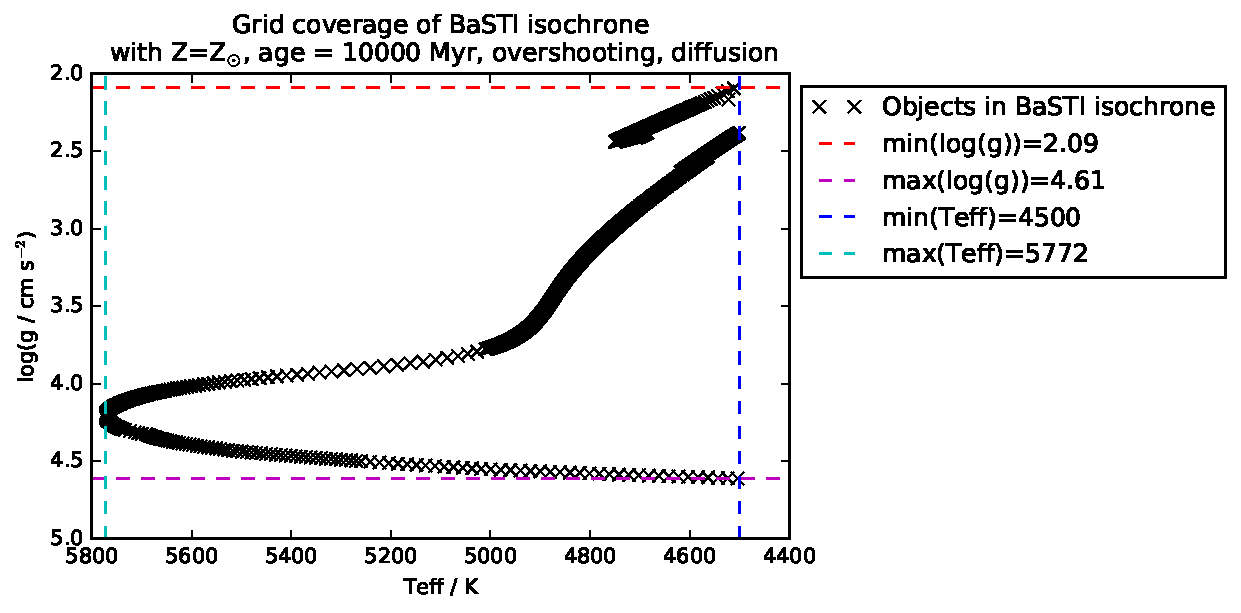
\includegraphics[scale=0.4]{../wfc3_16_23Myr_10Gyr_complex_solar/wfc3_ATLAS9_grid_BaSTI_coverage_c10000_complex_Zsol_4500.pdf}
\caption{$T_{\textnormal{eff}}$-log($g$) grid coverage by a 10 Gyr, $Z_{\odot}$ BaSTI isochrone ****including mass-loss, core overshooting and diffusion effects}
\label{BaSTI_coverage_10G}
\end{figure}

\begin{figure*}
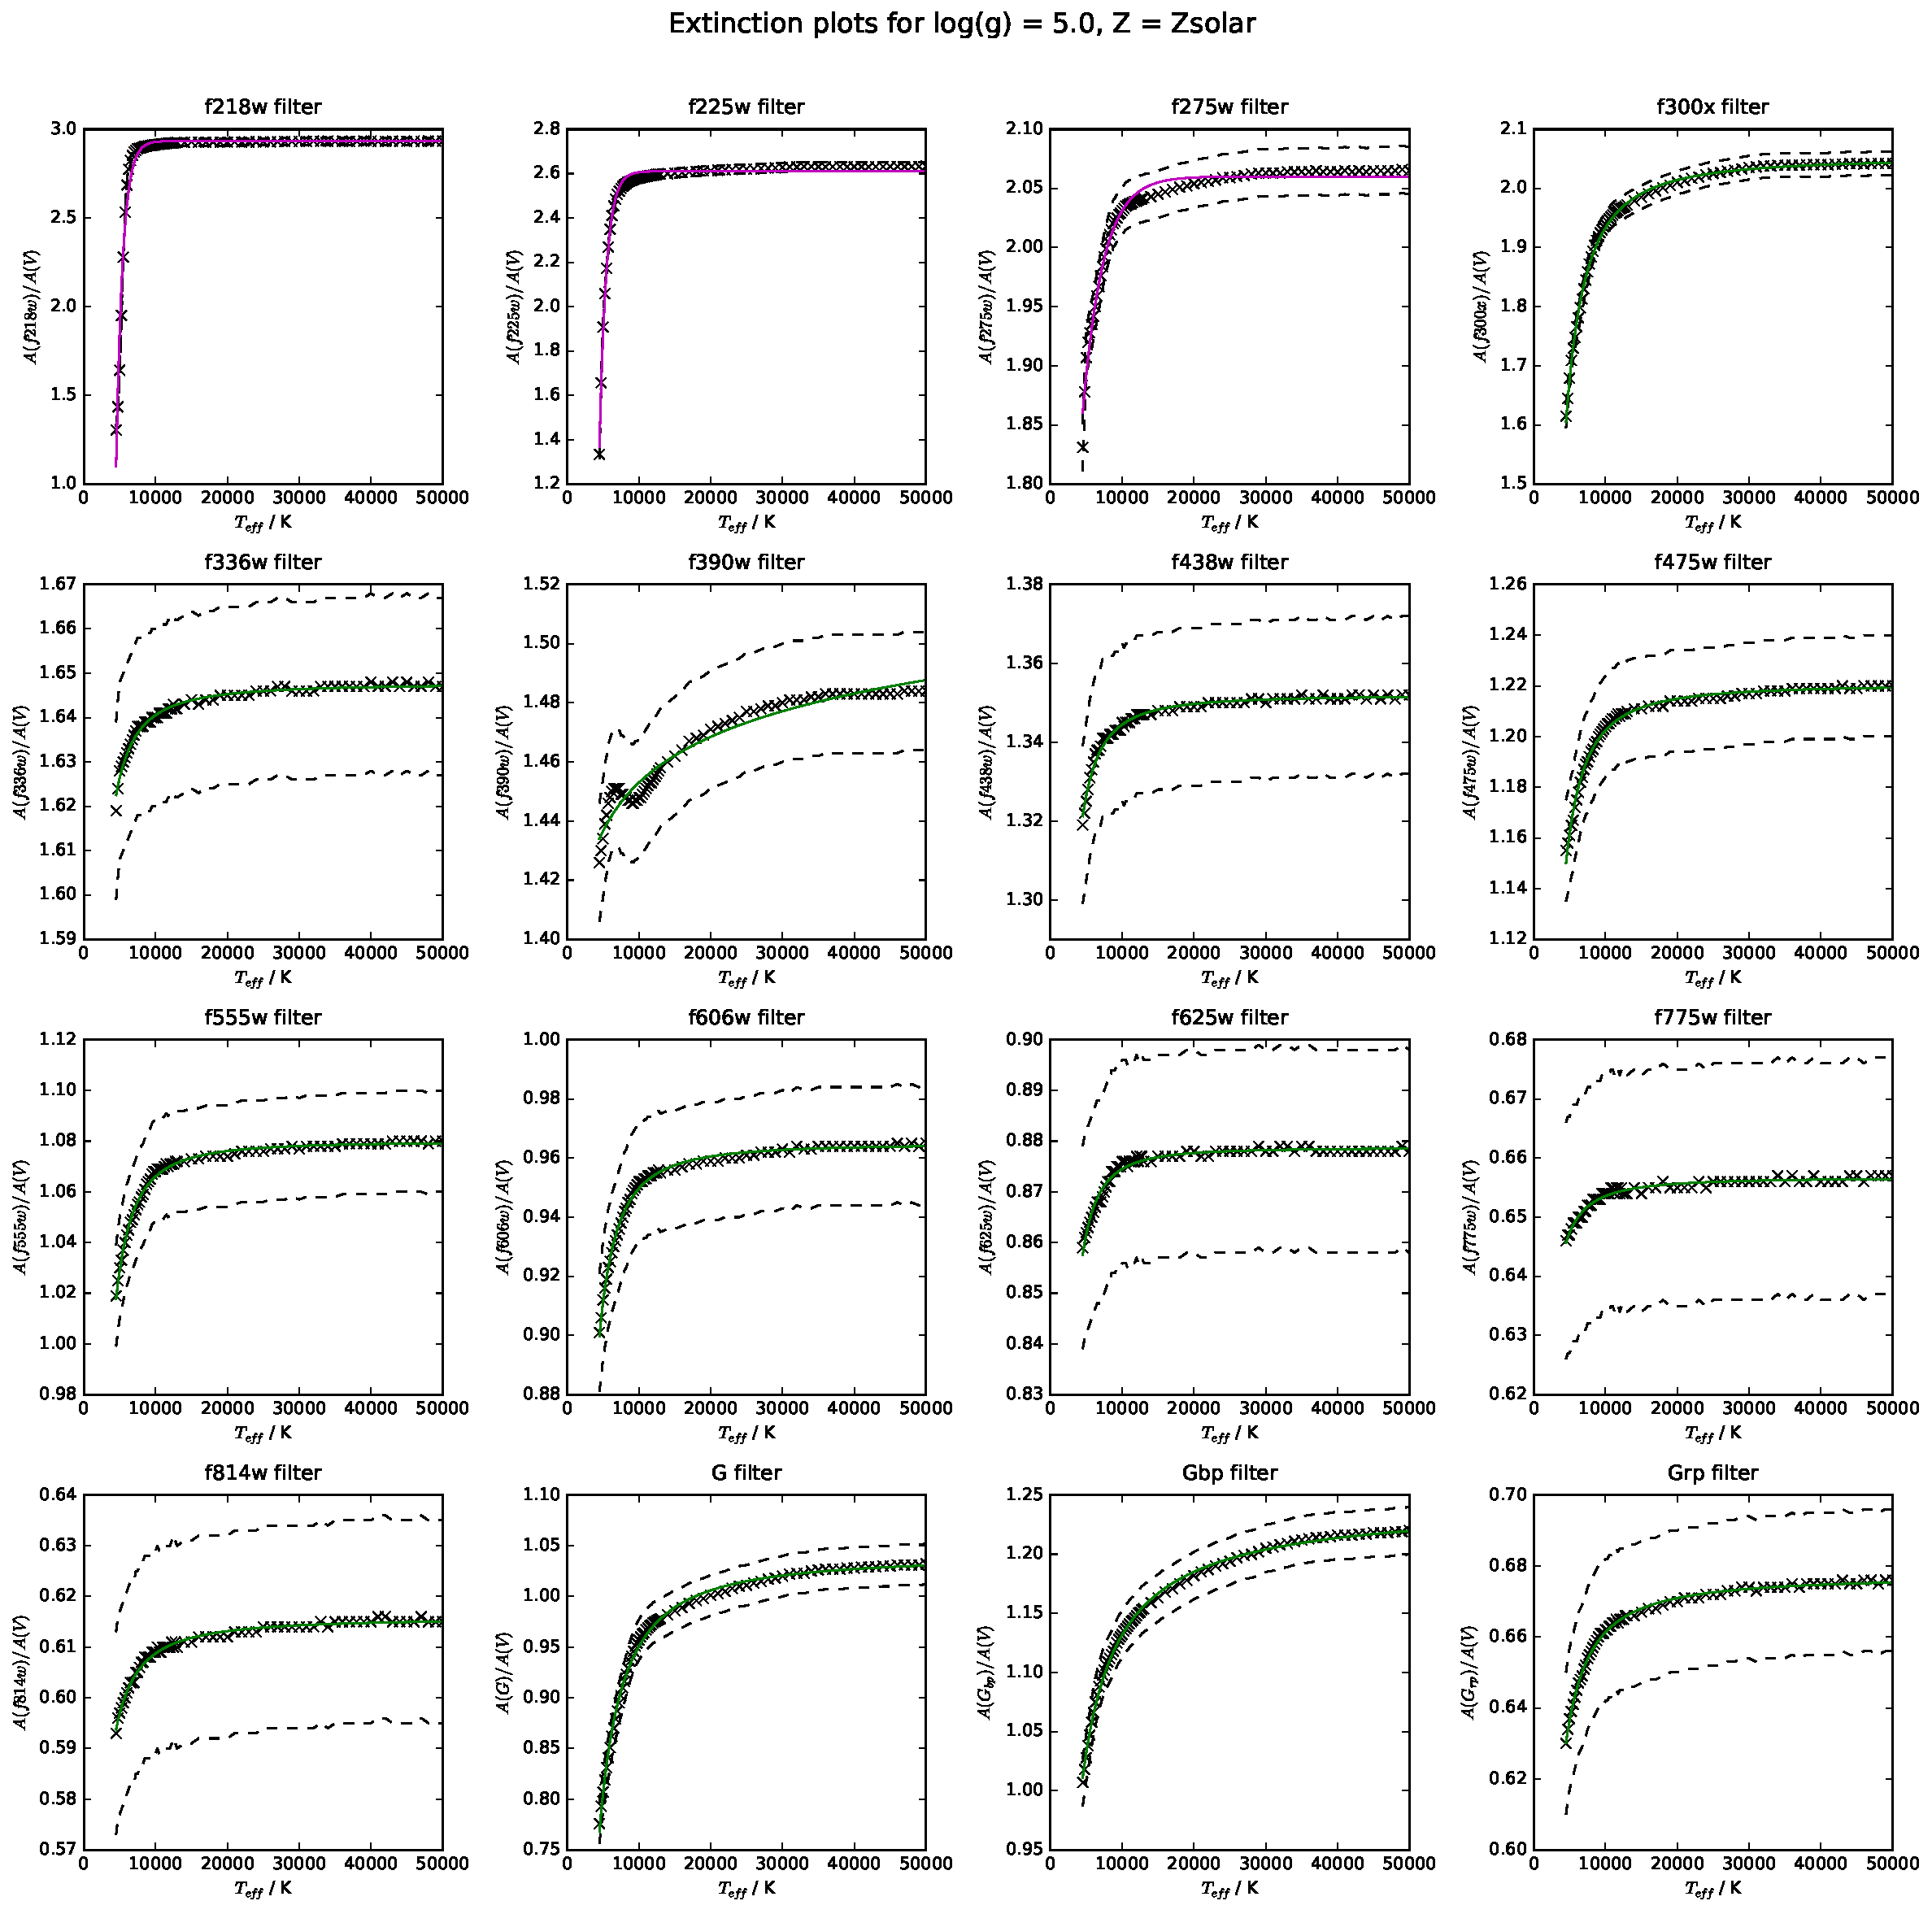
\includegraphics[scale=0.4]{../HubWFC/Hub_graphs/AHub_logg=5p0_solar_4500K_R1_only_Teff_fit_modded_plot.pdf}
\caption{Plots of the best $A_{1}$ fitting result in each filter. Purple lines indicate that the fit took the form $A_{1,\textnormal{exp}}$, while green lines indicate the same for $A_{1,\textnormal{pow}}$. The dotted lines indicate deviations of $\pm$0.02 from the data (black crosses)}
\label{R1_bests}
\end{figure*}

% ****FORMAT FOR INCLUDING PDF IMAGES!!!
% for guidance, see phd_work/grfguide.pdf
%\includegraphics[<options>]{filename.pdf}

\chapter{Discussion}
\section{Thermohaline mixing}
As shown in Figure \ref{dXN14/dt_colour}, the conditions for thermohaline mixing are reproduced in the BaSTI code. The location of the regions for which these conditions apply is located in the upper, and therefore cooler, layers of the hydrogen fusion shell,

So far, by measuring abundances of species which both are hydrogen fusion products and are not involved in $^{3}$He burning, such as $^{14}$N, it has been established that the existing BaSTI stellar evolution model creates the conditions for thermohaline mixing to occur in the radiative zone of a low-mass, post-FDU RGB star. It has also been shown that, as expected, the conditions are created by molecular weight inversions arising from $^{3}$He burning.

While the physical process and impacts of thermohaline mixing have been successfully implemented in other stellar evolution codes, such as MESA and STAREVOL, BaSTI has not yet been modified to include these in the iterative calculations. Achieving this is a significant goal because, as demonstrated by \cite{2015MNRAS.446.2673L} in the particular case of lithium abundances, there can be significant differences in predictions of abundances between different stellar evolution codes. Adding BaSTI to the list of codes available for future comparative studies would provide more scope to study potential sources of error, such as the model time-step and $C_{thl}$ value effects on abundances noted by \cite{2015MNRAS.446.2673L}. Of particular interest is the $C_{thl}$ free-parameter value, as there are many proposed values, from authors using different approaches and models, which differ in some cases by at least an order of magnitude.

While the magnitude of the thermohaline mixing effect in Figure \ref{dXN14/dt_colour} gives

\section{Differential extinction}
When fitting the $A_{1}$ functions, with the exception of the f218w, f225w, f275w and f300x filters (the shortest-wavelength filters, all in the UV), all fitting results were accurate to within $\pm$0.02 of the $\log(g) = 5.0$ data. From Figure \ref{all_Z_Z2_ratio}, the same pattern occurs with metallicity, as the data for only the 4 aforementioned filters vary by more than 3$\%$, even between the $\log(Z/Z_{\odot}) = -2.0$ and $0.5$ data.
The 4 filters with low-accuracy results will require additional terms in $T_{\textnormal{eff}}$, i.e. a modified  $A_{1}$ function, to mimic the data to an acceptable degree of accuracy
As shown in Figures \ref{BaSTI_coverage_16M} and \ref{BaSTI_coverage_10G}, even when considering only BaSTI isochrone data with $T_{\textnormal{eff}} \geq 4500$K, the range of log($g$) values covered still requires $A_{2}$ functions to be computed for the full range of isochrone ages, for those filters which require it, as shown by the significant changes in Figure \ref{all_logg_logg5_ratio}, even for log($g$) = 2.5, which is inside the lower limit for the 10Gyr isochrone. The relative shapes of the individual curves suggests that a single function of log($g$), moderated in magnitude by the $T_{\textnormal{eff}}$ of the data, could be obeyed by all of the curves. At the time of writing, this scenario is being studied using multiple forms of $A_{2}(T_{\textnormal{eff}},\log(g))$ below temperatures of 8000K. This apparent disagreement with the fitting function form described in \cite{2018MNRAS.475.5023C} and \cite{2018MNRAS.479L.102C} is simply due to the fact that the relevant filters were not studied in those works - this project agrees with those works for the filters studied both in those works

The significant effect of metallicity is also, at the time of writing being investigated using $A_{2}$ functions, as this effect also occurs in the region $T_{\textnormal{eff}} \leq 8000$K.

\chapter{Future work}
This work, although confirming feasibility of thermohaline mixing in BaSTI, has yet to implement the effects of the resultant chemical mixing on the models of the star at times following the initial mixing. The next step should be to integrate the conditions for thermohaline mixing into the relevant BaSTI routines allow local chemical compositions to change in response to thermohaline mixing, which in turn allows the mixing effect to propagate into the radiative zone, the first step that must be taken if the mixing is to have any impact on observable chemical abundances (i.e. at the stellar surface).

**** modelling/integrating other effects into BaSTI
The accuracy of the results of a full implementation of thermohaline mixing into BaSTI will still be unclear, given the known impact of rotation (\cite{1963ApJ...138.1134C} \cite{1998A&A...334.1000M},\cite{2017A&A...606A..55M},\cite{2012A&A...537A.146E}) and radiative levitation \citep{2016A&A...592A..29M} on stellar interior structure, and hence on observed emission, both in single stars  and populations. For example, rotation is a possible explanation for the phenomenon of extended main sequence turnoffs (\cite{2015MNRAS.453.2070N}, \cite{2016MNRAS.460L..20B}), split main sequences and multiple populations. If interior mixing effects are not included in calculations
%\cit

For differential extinction, the immediate goal is to derive $A_{1}$ and $A_{2}$ functions that are  sufficiently accurate. The final step will be to apply them to the isochrone data by using the values of $T_{\textnormal{eff}}$ and log($g$) for each object in a given isochrone, together with the $Z$ value of the isochrone and the unique coefficients for each filter. The resulting extinction will then be added to the filter magnitude data for the objects and colour-magnitude diagrams (CMDs) will be plotted, simulating an observed stellar population, to study any differences in the distribution of the objects. The final step will be to compare the results with observed populations in the same CMD.

The ultimate goal of this PhD, and of the field of stellar physics in general, is to predict, quantitatively and accurately, the evolution of a star and, particularly, its fundamental observable properties over the course of its lifetime. This requires all known potential sources of mixing and instability to be factored into a single framework. This project will attempt to work towards this goal in BaSTI.****

\chapter{Conclusion}
In this project so far, the physical conditions required for thermohaline mixing in low-mass RGB stars have been confirmed, and the projected effect of the mixing has been shown to be significant with regard to the local mass fraction of $^{14}$N.****

\chapter{Timeline}
****dgtfhfyhfy

\bibliographystyle{mnras} % unsrtnat
\bibliography{transfer_report}

\end{document}